%%%%%%%%%%%%%%%%%%%%%%%%%%%%%%%%%%%%%%%%%%%%%%%%%%%%%%%%%%%%%%%%%%%%%%%%%%%%%
%%%
%%% File: utthesis2.doc, version 2.0jab, February 2002
%%%
%%% Based on: utthesis.doc, version 2.0, January 1995
%%% =============================================
%%% Copyright (c) 1995 by Dinesh Das.  All rights reserved.
%%% This file is free and can be modified or distributed as long as
%%% you meet the following conditions:
%%%
%%% (1) This copyright notice is kept intact on all modified copies.
%%% (2) If you modify this file, you MUST NOT use the original file name.
%%%
%%% This file contains a template that can be used with the package
%%% utthesis.sty and LaTeX2e to produce a thesis that meets the requirements
%%% of the Graduate School of The University of Texas at Austin.
%%%
%%% All of the commands defined by utthesis.sty have default values (see
%%% the file utthesis.sty for these values).  Thus, theoretically, you
%%% don't need to define values for any of them; you can run this file
%%% through LaTeX2e and produce an acceptable thesis, without any text.
%%% However, you probably want to set at least some of the macros (like
%%% \thesisauthor).  In that case, replace "..." with appropriate values,
%%% and uncomment the line (by removing the leading %'s).
%%%
%%%%%%%%%%%%%%%%%%%%%%%%%%%%%%%%%%%%%%%%%%%%%%%%%%%%%%%%%%%%%%%%%%%%%%%%%%%%%

\documentclass[a4paper, 12pt, oneside]{report}         %% LaTeX2e document.
\usepackage {tcdthesis}              %% Preamble.
\usepackage{graphicx,color}
\usepackage{anysize}
\usepackage{nth}
\usepackage[table]{xcolor}
\usepackage{array,ragged2e}
\usepackage{amsmath}
\usepackage{longtable}
\mastersthesis                     %% Uncomment one of these; if you don't
%\phdthesis                         %% use either, the default is \phdthesis.

\thesisdraft                       %% Uncomment this if you want a draft
                                     %% version; this will print a timestamp
                                     %% on each page of your thesis.

\leftchapter                       %% Uncomment one of these if you want
%\centerchapter                      %% left-justified, centered or
% \rightchapter                      %% right-justified chapter headings.
                                     %% Chapter headings includes the
                                     %% Contents, Acknowledgments, Lists
                                     %% of Tables and Figures and the Vita.
                                     %% The default is \centerchapter.

% \singlespace                       %% Uncomment one of these if you want
% \oneandhalfspace                   %% single-spacing, space-and-a-half
 \doublespace                       %% or double-spacing; the default is
                                     %% \oneandhalfspace, which is the
                                     %% minimum spacing accepted by the
                                     %% Graduate School.

\renewcommand{\thesisauthor}{Samuil Hristov}            %% Your official UT name.
\renewcommand{\thesismonth}{April}                  %% Your month of graduation.
\renewcommand{\thesisyear}{2019}                      %% Your year of graduation.
\renewcommand{\thesistitle}{\tiny{} \\ \LARGE{Integration of Blockchain and Named-Data Networking}}            %% The title of your thesis; use mixed-case.
\renewcommand{\thesisauthorpreviousdegrees}{ }  %% Your previous degrees, abbreviated; separate multiple degrees by commas.
\renewcommand{\thesissupervisor}{Dr. Stefan Weber}      %% Your thesis supervisor; use mixed-case and don't use any titles or degrees.
% \renewcommand{\thesiscosupervisor}{}                %% Your PhD. thesis co-supervisor; if any.

% \renewcommand{\thesiscommitteemembera}{}
% \renewcommand{\thesiscommitteememberb}{}
% \renewcommand{\thesiscommitteememberc}{}
% \renewcommand{\thesiscommitteememberd}{}
% \renewcommand{\thesiscommitteemembere}{}
% \renewcommand{\thesiscommitteememberf}{}
% \renewcommand{\thesiscommitteememberg}{}
% \renewcommand{\thesiscommitteememberh}{}
% \renewcommand{\thesiscommitteememberi}{}

\renewcommand{\thesisauthoraddress}{Dublin, Ireland}

%\renewcommand{\thesisdedication}{...}     %% Your dedication, if you have one; use "\\" for linebreaks.


%%%%%%%%%%%%%%%%%%%%%%%%%%%%%%%%%%%%%%%%%%%%%%%%%%%%%%%%%%%%%%%%%%%%%%%%%%%%%
%%%
%%% The following commands are all optional, but useful if your requirements
%%% are different from the default values in utthesis.sty.  To use them,
%%% simply uncomment (remove the leading %) the line(s).

% \renewcommand{\thesiscommitteesize}{...}
                                     %% Uncomment this only if your thesis
                                     %% committee does NOT have 5 members
                                     %% for \phdthesis or 2 for \mastersthesis.
                                     %% Replace the "..." with the correct
                                     %% number of members.

\renewcommand{\thesisdegree}{Bachelor of Arts(Mod.)}  %% Uncomment this only if your thesis
                                     %% degree is NOT "DOCTOR OF PHILOSOPHY"
                                     %% for \phdthesis or "MASTER OF ARTS"
                                     %% for \mastersthesis.  Provide the
                                     %% correct FULL OFFICIAL name of
                                     %% the degree.

\renewcommand{\thesisdegreeabbreviation}{B.A.(Mod.)}
                                     %% Use this if you also use the above
                                     %% command; provide the OFFICIAL
                                     %% abbreviation of your thesis degree.

\renewcommand{\thesistype}{Dissertation}    %% Use this ONLY if your thesis type
                                     %% is NOT "Dissertation" for \phdthesis
                                     %% or "Thesis" for \mastersthesis.
                                     %% Provide the OFFICIAL type of the
                                     %% thesis; use mixed-case.

% \renewcommand{\thesistypist}{...}  %% Use this to specify the name of
                                     %% the thesis typist if it is anything
                                     %% other than "the author".

%%%
%%%%%%%%%%%%%%%%%%%%%%%%%%%%%%%%%%%%%%%%%%%%%%%%%%%%%%%%%%%%%%%%%%%%%%%%%%%%%



\begin{document}                                  %% BEGIN THE DOCUMENT
\begin{titlepage}
\begin{center}
\huge{University of Dublin}\\[2.5mm]
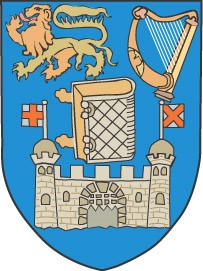
\includegraphics[width=1.2in]{trinity.jpg}\\
\Huge{TRINITY COLLEGE} \\
\vspace{1in}
\Large\textbf{Integration of Blockchain and Named-Data Networking}\\
\vspace{0.5in}
Samuil Hristov\\
Final Year Project April 2019\\
Supervisor: Dr. Stefan Weber\\
\vfill
School of Computer Science and Statistics\\
O'Reilly Institute, Trinity College, Dublin 2, Ireland\\
\end{center}
\end{titlepage}
\thesisdeclarationpage				  %% Generate the declaration page.

\thesispermissionpage				  %% Generate the copyright permission page

%\thesisdedicationpage                             %% Generate the dedication page.

\begin{thesisacknowledgments}                     %% Use this to write your
 todo
\end{thesisacknowledgments}                       %% allowed in LaTeX2e par-mode.

\begin{thesisabstract}

\textbf{Abstract:} Information-Centric Networking (ICN) is a communication approach that 
makes content 'living' in a network the focus of communication, in 
contrast to the traditional communication between hosts based on IP 
addresses. In order to ensure the validity of content, it should be 
signed by its producer and  in order to ensure that information is only 
accessible to a select number of consumers, content may need to be 
encrypted. Named-Data Networking (NDN) is an ICN implementation that 
provides a framework for the exchange of named content and a 
certificate-based security mechanism to sign and encrypt/decrypt 
content. The certificates in NDN are held at individual nodes and have 
to be requested by other nodes in a network in order to verify content, 
leading to additional latency once content has been retrieved.

This project has extended NDN's certificate management system by 
distributing certificates based on a distributed ledger i.e. a 
blockchain. Transactions such as the creation and removal are announced 
by nodes to miners which incorporate the transaction into new blocks and 
distribute these to nodes for inclusion into the Blockchain. Nodes have 
access to the current set of certificates through their Blockchain and 
can verify content through these certificates.

NDN currently implements a signature verification standard by defining a common certificate format. All signed data transfers in NDN are certificates because they contain a public key.X509 Format.
\end{thesisabstract}

\tableofcontents                                  %% Generate table of contents.
\listoftables                                     %% Uncomment this to generate list of tables.
\listoffigures                                    %% Uncomment this to generate list of figures.

%%
%% Include thesis chapters here...
%%
  \chapter{Introduction}
Named Data Networking is an interesting new paradigm in the space of network architectures. Years on since Bell Labs' work on telephony, networking research assumed that telephony is the right model for data networking[1]. This model implied that there had to be a determined route between two points for communication to happen - the setup for which was costly. This was proven not to be the case in Paul Baran's research paper titled "On Distributed Communication Networks" in 1964, which was widely disregarded until the practical application of his work in ARPAnet(Sept,'71).MIT Senior Researcher David Clark's paper on end-to-end principle confirmed the same and it became apparent that networking solved the telephony problem. However, we are still using this same architecture which was invented as a solution for a problem of 5 decades ago, and the Internet of today is not facing the same challenges. CISCO predicted in 2013[C.Index, Iouannou+Weber], that by the end of 2017, the annual traffic of the internet would exceed 1.4 zettabytes with almost 80\% of that being video traffic.

This is why, in the age of content delivery, Named Data Networking and other Information Centric Networking architectures aim to move away from the source-destination pairwise method of IP communication which is inherently limited. Instead, NDN proposes a Name-based approach where each node in a network can require content based on the name of the piece of data it requires. 

This project aims to improve on the security implemented in Named Data Networking.


The aim of this introduction is to give background for motivation as well as lay out the structure of this paper.
\section{Motivation}
Traditional NDN: The traditional NDN architecture presents a security architecture not dissimilar to the Central Authority architecture conceptualized by Loren Kohnfelder in 1978[cit]. It provides a public file[cit] system where all nodes can check the entries for other nodes issued by a Central Authority which signs each entry(certificate). 

\section{Aims}
Instead of transactions, this project aims to store certificates in a similar fashion. The goal is to do so efficiently, without increasing computational load on individual nodes in the system or increasing significantly the bandwidth use.

 It is important to note that there isn't a monetary incentive for doing this "Proof-of-Work"[2] so each network should have a dedicated group of miners which verify blocks. The assumption here is that all(or most) of the nodes will not be malicious and will not be pooling their resources to attack the network. This means that in order for one to alter the list of certificates, they would have to have more computing power than the entire network of miners. This will allow for safer communication between nodes in a network. 
\vfill
\section{Road-map}
\chapquote{``Begin at the beginning," the King said gravely, ``and go on till you come to the end: then stop."}{Lewis Carroll}{Alice in Wonderland}

This paper is structured as follows: State of the Art(Lit. Review), Design and Implementation, and Evaluation.
\begin{itemize}
\item Chapter 2 contains the literary reviews of the papers which discuss the State of the Art. It looks at a ranking system for the papers reviewed and also provides critique for each one. 

\item Chapter 3 discusses in detail the design and implementation of the Blockchain solution in NDN. It outlines all aspects of the practical work, including solutions, design challenges and alterations that were made along the way.

\item Chapter 4 goes on to evaluate the working solution by discussing different experiments and topologies. It presents graphs which illustrate the performance differences in different topologies
\end{itemize}
The paper's conclusion then sums up the work that's been presented and outlines any future work that might be undertaken regarding the project.                                
  \chapter{State of the Art}
\section{{Introduction}}
The State of the Art in NDN and Blockchain was thoroughly investigated when researching this project. This was done to establish what technologies are currently implemented in Named Data Networking and also to identify similar projects to our own solution.\par It is important to note this was done to a lesser extent for Blockchain because it is a supplemental technology in the Cryptocurrency space and is relatively simplistic(i.e. a vector of blocks all hashed with the previous block's hash).The Blockchain "itself requires minimal structure"[3 - nakamoto] Therefore, the different nuances of the technology which deviate from the fundamentals weren't investigated as thoroughly as it was beyond the scope of the project specification which asked for a proof of concept Blockchain. This involves miner nodes solving basic proof of work or cryptographic puzzles[3 - nakamoto], based on a timestamped transaction, appending them to a chain, and advertising that chain to all nodes in the network. 

This chapter is divided into Knowledge and Literary Review sections. The knowledge contextualizes this project by giving in depth background on all the technologies in use. 

The Literary Review then describes each individual paper from which this information was obtained. 

\section{Background and Summary}
In 2006, Van Jacobson likens the ICN solution for the IP problem to the Copernican solution for the Solar System problem.[4 - van google videos] What he suggests by saying this is that IP was a(good) solution but for an entirely different problem than what the Internet is today. "While it is entirely doable to predict the movement of planetary bodies by taking the Earth to be the center of the universe, it is incredibly complex. This is because the point-of-view is wrong." [4 - van google videos] Dissemination Networking.

The background for this research splits off into two parts. The Blockchain technology is largely based on cryptography and hashing. NDN on the other hand has its roots in networking. 

The following table aims to quantify the usefulness of each paper that has been looked at. This method has been directly inspired by Masters student Conor Mooney who did an excellent job at scoring and qualifying his papers while researching. The categories for each paper reviewed fall under one of three categories: analysis, implementation, review.\\
\begin{itemize}
\item Analysis - Refers to papers which analyse a technology\\
\item Implementation - Refers to papers which discuss technical aspects of the technologies which were used. These papers were mostly the NDN Developer Guides.\\
\item Review - Reviews classify papers which mainly contribute with an evaluation - useful when there are different technologies that one might use for a particular problem, allowing for the narrowing down of solutions.\\
\vfill
All papers will be scored based on a retroactive relevancy heuristic i.e. how useful did these papers end up being to the problems presented in this project. 
\end{itemize}
\begin{table} [!htb]
\caption{Relevancy of Papers}
\centering
\begin{tabular}{l|c|c}
Paper & Type & Score \\ 
V. Jacobson - Networking Named Content & Analysis & 5\\
D. Kim - Efficient and Secure NDN & Implementation & 5\\
S. Weber - Caching & Implementation & 3\\
K. Lei - Blockchain Based Key Management & Implementation & 5\\
L. Zhang - Named Data Networking & Review & 4\\
S.Nakamoto - Bitcoin & Implementation & 4 \\
L. Zhang - NDN & Implementation & 4 \\
K. Huang - Cyber Attack Business & Review & 3 \\  
K. Lei - BlockNDN & Implementation & 5 \\ 
L. Wang - NLSR & Implementation & 5 \\ 
NFD Team - NFD Developer's Guide & Implementation & 4 \\ 
A. Afanasyev - NDN Technical Report 9 & Implementation & 4 \\ 
Y. Yu - NDN Delorean & Implementation & 4\\
S. Mastorakis - Security Support in NDN & Implementation & 5\\
Diffie \& Hellman - Privacy and Authentication & Implementation & 3 \\
R. Merkle - Protocols for PK Cryptosystems & Review & 3 \\
Kohnfelder - Central Authority & Implementation & 3

\end{tabular}
\end{table}
\section{State of The Art - Knowledge}
\subsection{Blockchain}
Blockchain is a distributed ledger of immutable digital records[medium.com]. It was conceptualized in Satoshi Nakamoto's Bitcoin paper in 2009. It is the main component of the Bitcoin cryptocurrency. It allows for decentralized transactions by solving the Byzantine Generals Problem[cit].\par 
This problem refers to the inability of traditional systems, without a central authority, to determine that a certain resource hasn't been spent more than once. The reason banks or "central authorities" can vouch for transactions, and guarantee against double spending, is because the transactions don't happen instantaneously. They are each, individually confirmed, and also, should the bank make a mistake, it covers it(insurance).\par 
The reason this isn't the case in a Blockchain distributed ledger system like Bitcoin, is because miners do Proof-of-Work on each node before verifying a transaction.
\begin{figure}
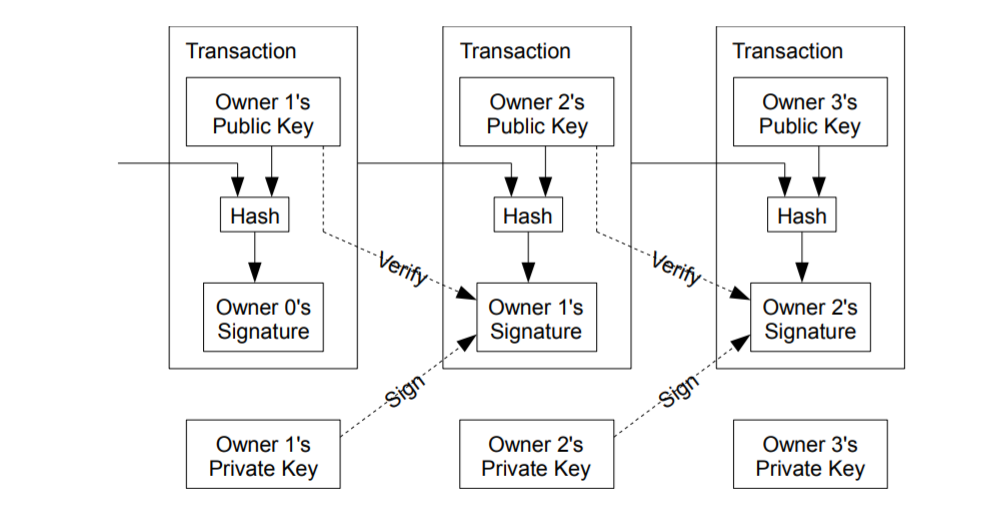
\includegraphics[width=6in]{hashes.png}
\caption{Blockchain structure[satoshi]}
\end{figure}

\subsection{NDN}
Named Data Networking began life in 2010 under the NSF's Future Internet Architecture[cit-ndn-tutorials-sigcomm17]. The leading effort in the NDN project has been UCLA Professor Lixia Zhang. Projects like NDN picked up traction after CCN began development at PARC, headed by Van Jacobson. NDN presents a paradigm shift for the Networking Stack. Instead of IP being the thin-waist of the stack, NDN suggests a data name abstraction, where the name of the content becomes this thin-waist. \par
NDN is composed of a number of modules described below. It is a name based architecture where nodes in a network can request data, not based on where it comes from but based on the name of the data. I.e. a node requests /ndn/a-site/important/information instead of an IP address. This abstraction is hugely advantageous in today's Internet where content sharing is at the forefront of what the Internet delivers. NDN allows for nodes to respond to content requests(Interests) with Data packets. Nodes interact by sending Interests by Name. Data is retrieved in Data packets.\par 
\vfill
\begin{figure}
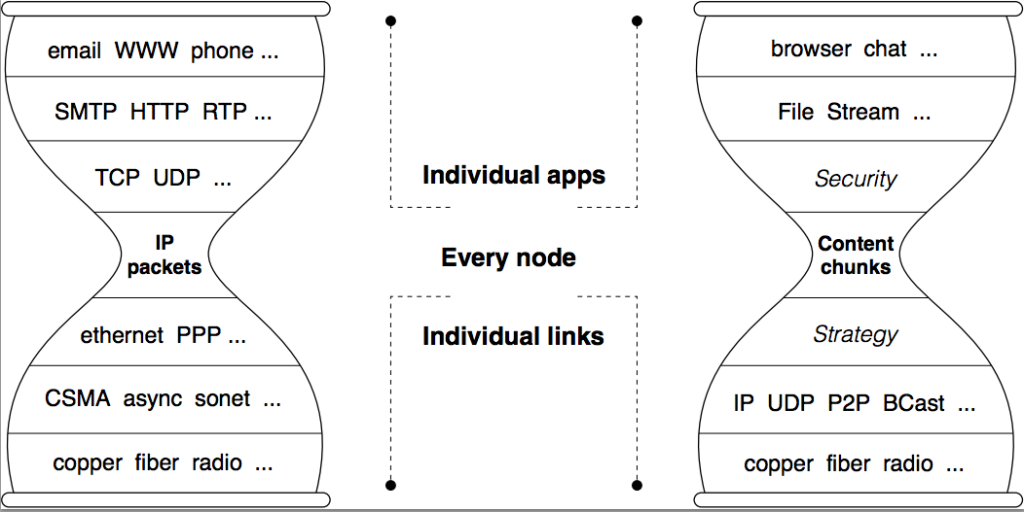
\includegraphics[width=6in]{hourglass.png}
\caption{The Networking Stack}
\end{figure}
\subsection{Names}
An NDN Name is a hierarchical name for NDN content, which contains a sequence of name components.[named-data.net docs] Each NDN name component  consists of variable lengths and is separated by a '/' separator. This design is advantageous because it is human readable and allows for users to configure Interest and Data filters using regular expressions. \\
E.g: InterestFilter$(^<ndn><lectures>)$ means listen for any interests beginning with /ndn/lectures. 
Named Data Networking is all about names. When presenting on NDN at MILCOM 2017 in Baltimore, Lixia Zhang said "the secret to NDN is in the names!" This is because this networking paradigm  is entirely centered on the names of content. Each entity in a network has an identity, and each identity has a name. Each named entity in a network follows a hierarchical naming scheme.\par
Names are represented by the name class in NDN. They are made up by a URI string. In C++, they are defined using the C-style const char* array. \par
Packets are forwarded using Longest Name Prefix Matching(LNPM).[Yuan] 

It is similar to IP Longest Prefix Match where a routing algorithm will, upon needing to do a look-up, return the longest matching address. E.g:
Consider the following IPv4 Forwarding Table(CIDR Notation):\\
192.168.20.16/28\\
192.168.0.0/16\\
If the router was to look-up 192.168.20.19, both entries will "match", but the router will only return 192.168.20.16/28 since the submask /28 is longer than the other entry's /16 submask. [example-wikipedia]

A similar example could be given an Interest arriving at node B asking for /ndn/a-site/lectures/telecomms/slides  and node B's FIB could have entries for /ndn/a-site and /ndn/a-site/lectures/telecomms/ in which case it will only return the second entry. \par 

The problem with LNPM comes from the inherent differences between address lengths in IP and NDN. In most cases, NDN names will be longer than IP as the namespace is unbounded. The difference in size is so drastic, that TCAM or SRAM memory modules for the FIB would not be large enough if the number of rules is large. The NDN FIB has to use DRAM in order to accommodate for this size difference. With such a difference in size and complexity, look-ups can take O(k) string look-ups[yuan].\par 
This is why NDN employs two techniques proposed in a Washington University paper by Haowei Yuan and Patrick Crowley. The first changes the LNPM design to a binary search of hash tables reducing lookups to O(log(k)) for prefixes with k components [yuan] and the second technique is level pulling to improve the average case. This makes the name prefix lookup solution scalable - a necessary feature for the NDN architecture to work. 

\subsection{NFD}
Named Data Forwarding Daemon is responsible for handling all packets in the network. An instance of NFD runs on every node in a network. When a packet arrives the NFD checks if that packet is destined for the particular node and if not it discards it based on a policy to allow/disallow unsolicited Data packets.
\subsection{NLSR}
Named Data Link State Routing is the NDN module which deals with routing when a topology is created. NLSR works by sending out Link State Advertisements when a network is created. What this means is that, each node has its Forwarding Interest Base populated with adjacent nodes. NLSR takes time to converge proportional to CPU power in the Network. 
\subsection{Chronosync}
Chronosync is a module used when there is a need for nodes to receive data or be updated at the same time. Chronosync runs on top of NFD and synchronizes Data and Interest packet sending and receiving.
\subsection{Content Store}
The Content Store or cache is each node's local storage. It contains signed Data which the node can forward to any node expressing an interest for it. Caching is one of NDN's main features. There are two types - off path and on path caching. Off path caching, like the name suggests, disregards content path and just aims to replicate the content in a network[weber, ioannou]. On Path caching is limited to the content propagated along the delivery path[weber,ioannou] meaning the data cannot be cached outside the route from the node expressing the Interest for the Data and the producer of said Interest.
\subsubsection{Policies}
A number of policies exist for caching:FIX(0.9), DC and ProbeCache. A recent solution - ProbPD investigates content popularity as a heuristic for caching. All of the high-end solutions perform near identically.
\subsection{Security}
Ralph Merkle describes the problem with the classic[cit] Authenticated Public Key Distribution protocol. He describes how each node in a network generates a public key and stores it in a file system. If two nodes wish to agree on a common key in order to interact, they look up the Public Key portion of the other node. Then each send a \textbf{session key} encrypted with the other node's public key. Once in agreement, this key is secret and authenticated and can be used by both nodes to communicate. 

The problem with this approach is that a centralized file system is a single point of failure and is prone to attack. The attacks can be one of two - the public key elements can be altered in the file system(e.g. the attacking node could set another node's public key to be its own), and secondly, the private keys can be lost.

 The alternative to this approach is implemented in NDN and it is to introduce Certificates and a Certificate Authority(CA). Certificates refer to the binding of a node's keys to its identity i.e. which key belongs to which node. It is very important that there is a robust method of determining this key-identity bond and perhaps even more importantly, to ensure that it is immutable. "In NDN, every entity that produces data needs to obtain an NDN certificate to prove the ownership of its namespace and cryptographic materials(public key)"[spyridon].
 The security process occurs as following: First, we start off with the Achilles Heel for any networking security protocol - \textbf{bootstrapping}. This is the process of obtaining all trust anchors and certificates. 
	 
 Before that however, we need to just quickly define trust anchors(policies). They refer to the rules set by each entity to only accept packets of a desired format of names and name relationships[spyridon]. It is also important to note that these rules are governed by each identity at the Application Layer.
 
  Back to bootstrapping: In order to do this, nodes must obtain a namespace and then a certificate for that namespace from a CA that they trust.[spyridon] The order for entities receiving certificates is hierarchical. This means that if a user(entity) has obtained a certificate, it can delegate certificates to other entities within its namespace.
 Because trust anchors are determined at the Application Layer - the only prerequisite[spyridon] for security bootstrapping is allocating names. As long as an entity has a name, it can receive a certificate if allowed by the owner of the namespace. 
 Each entity has its own trust anchors but should naturally trust the Certificate Authority. In the case of the root namespace - that is the recognized CA by the root user, as for the rest of the names in the namespace, that is the root namespace.\par
 \textbf{NDNCERT} is a library found in NDN-CXX which provides the tools necessary for a name to obtain a certificate in an NDN network. It generates certificates for trust anchors automatically and manages them in a daemon[spyridon]. It runs in an instance called an agent and maintains all certificates generated by NDNCERT.\par
As well as that NDNCERT can revoke certificates automatically if they are considered unfit. There is a check done on each certificate and if it is generated illegally, then in the case of the MiniNDN emulator, the code will throw an error and exit the session.\par
Data packets are signed at creation time[spyridon]. This design choice is critical in the integrity of data packets in NDN because this means that a data packet physically cannot be sent off without being signed. The important bit here isn't so much that all data sent is signed as much as is the inverse - that all data received can be checked for a signature. 

This makes Data verification twofold: Firstly, NDN uses Trust Anchors - so if a node is expecting data, it can define a trust anchor that states that the data can only arrive from one particular \textbf{name}. Secondly, and this is the traditional, cryptographic verification method, once the Data packet is received and passes the trust anchor check, the consumer of the Data packet retrieves the corresponding certificate for the producer which is identified by the key name section in the packet[spyridon]. The Certificate will then recursively point to the root certificate and if all certificates along the way are valid that means that the Data packet itself is signed with a valid signature.

\section{Related Work}
There are a number of papers that I've come across that deal with security in NDN. As expected, there is plenty of work done in this field because it is a major concern for any network architecture.\par 

The NDN guides were a big help when it came to researching security. Spyridon Mastorakis' paper on NDN Security Support outlines all major features found in the Security module of NDN. This paper cited the Merkle paper on Public Key Distrtibution with Tree Authentication which is what is currently used in NDN.\par



However, when it came to Blockchain integration in NDN, there wasn't much work done in the field. Hashing, on one hand, is a big part of NDN security because of the size of NDN Names as described above. To this degree, much of Ralph Merkle's work has been employed in NDN, but the Blockchain concept in general isn't seen much. 

There is one particular paper titled BlockNDN by Kai Lei which describes a Blockchain abstraction for use in IP using multicast. This paper investigated whether Blockchain is a good fit for NDN and although it did not present a security solution involving Blockchain, this investigation was very useful when designing the solution for this paper.\par

Another related solution which I used for some of its ideas was Alexander Afanasyev's paper titled NDNDelorean. This paper introduced a version concept for old data that needed to be authenticated. The version concept is quite useful when it comes to certificates. Because certificates can become invalid, it is important to be able to invalidate them. The problem with the Blockchain approach is that once appended to the Blockchain, a certificate can never be deleted without altering the whole Blockchain, which would render the whole Blockchain invalid. This is why, instead we introduce "version control" which in this project's case involves a simple integer(which could also be a boolean) which keeps track of a block's certificate's version. The current version is 1 if valid and 0 if invalid.
\section{Literary Review}
This section has been divided in the different technical components that I've investigated as part of my FYP. Apart from being split into NDN and Blockchain, I've also split NDN into: Security, NFD, NLSR, Mini-NDN, Content Store.

\subsection{Security}
[Kim15]Efficient and Secure NDN by D. Kim - 2015 Seventh International Conference on Ubiquitous and Future Networks, pp. 118-120, Tokyo, Japan. 7-10 July 2015.

This paper is important to my State of the Art review because it clearly outlines the current security challenges in Named Data Networks. It suggests a new way of implementing security protocols which currently are only implemented at the application layer and aren’t enforced. Because checking for which packets are signed at each packet transfer becomes recursive and very slow for any reasonable size transfer, this paper recommends only checking for signed data at critical points, incurring a smaller overhead on data transfer. This paper also presents an experiment on speeding up NDN by bundling Interest requests instead of burst firing interests for each packet. The paper concludes that this technique is upper-bounded by a $2^{\frac{1}{2}n}$ bundle size, yet delivers tremendous speed-ups in interests where the number of segments is larger than 4096.\par

[Mastorakis18] Security Support in Named Data Networking by Spyridon Mastorakis, Yanbiao Li, Lixia Zhang, Eric Newberry, Zhiyi Zhang, Haiteao Zhang, Alexander Afanasyev - NDN Technical Report, NDN-0057.

This paper was excellent for giving insight into NDN security. It described an implementation for NDNFit - an app which is designed to run on a user's phone or "data-collector". The user authenticates the collector to gather information, and then to encrypt and send that information to the user's laptop or "analyzer". The point of this implementation was the creation of a hierarchical trust model which employs not only cryptology but NDN's trust anchors to implement network security. The paper was very thorough in describing how a central authority(CA) authenticates certificates. It gives the NDNCERT library as an example of an authority which automatically verifies namespaces and trust anchors and signs certificates. Overall, this paper was extremely relevant to my work and very insightful into NDN security.

[Kohnfelder78] Towards a Practical Public-Key Cryptosystem - Loren Kohnfelder - MIT B.Sc. Dissertation

Despite the age of this paper, Kohnfelder gives a great overview of cryptographic techniques still used in cryptography today. Apart from his own contribution to the world of networking security, he also outlines mathematically, methods for encoding and decoding using cryptographic keys given in RSA, Diffie Hellman and Merkle. Most importantly though, in this paper, he introduces the concept of the certificate. It is this paper that recognizes the importance of a Certificate Authority, which is authorised to keep track and maintain a list of certificates(cryptographic entities) which guarantee that a a piece of content signed by a particular key is legitimately signed by that key. This sets the foundation for Merkle's paper on Certificate management.

[Merkle80] Protocols for Public-Key Cryptosystems - Ralph Merkle - 1980 IEEE Sysmposium on Security and Privacy

This paper is the natural evolution of the Kohnfelder paper. It also gives an overview of the broad scope of security solutions in place. Much like the Kohnfelder paper, despite its age, the techniques proposed are still in use today. Merkle describes different protocols and their benefits and drawbacks. He describes in depth: Simple Public Key Distribution, Authenticated Public Key Distribution, Public Key Distribution with Certificates, and Public Key Distribution with Tree Authentication. Merkle saw the potential of the certificates protocol and wanted to improve on it in this paper. He recognizes that despite the idea, the CA's decryption key is vulnerable to attack, which would result in system-wide loss of authentication. Merkle proposes a hashing function be used on the entire public file instead of the CA having to sign each entry in the Public File. This public file has a root which allows users in the network to use to derive the certificates. Once the nodes know the root, any attempt to alter the public file will now result in a different value for the root, which allows for easy detection. This paper directly builds on Kohnfelder's work and lays one of the foundations for network security implemented in NDN.  


\subsection{Overview}
[Jacobson09] Networking Named Content by Van Jacobson, D.K. Smetters, James D. Thornton, Michael Plass, Nick Briggs, Rebecca L. Braynard - In CoNEXT '09: Proceedings of the \nth{5} International Conference on Emerging Network Experiments and Technologies. Rome, Italy. 1-4 December, 2009.

The Van Jacobson paper on "Networking Named Content" is relevant to my State of the Art review, because it is the first paper to describe Content Centric Networking, on which Named Data Networking is based. This paper largely follows on from Dave Clarke's work in the field of the point to point communication problem. NDN is a direct evolution of both Clarke's work and Van Jacobson's work in CCN. It is implemented in much the same way, by fundamentally using very similar routing as IP, where nodes express Interests which are logged as faces in FIB tables for each NDN node, and are returned with a single Data packet over the shortest available path. "CCN is a networking architecture built on IP's engineering principles, but using named content rather than host identifiers as its central abstraction." NDN is also similar to CCN because it implements its 'soft state' model - meaning an expressed interest that isn't consumed by  a Data packet is timed out, therefore the machine expressing an Interest must re-express that interest if it still requires the data. In conclusion, this paper is the foundation of Named Data Networking, which carries over many of the proposed features in CCN in its State of the Art form, including its Node Model, Transport, Sequencing, Routing and Security.


\subsection{Content Store}
[Weber14]A Survey of Caching Policies and Forwarding Mechanisms in Information-Centric Networks by S. Weber, A. Ioannou - \nth{39} Annual IEEE Conference on Local Computer Networks. Edmonton, Canada, 8-11 September 2014.

The paper on Caching Policies and Forwarding Mechanisms was relevant to my work because it described in detail the current SOA of caching policies. As a survey, the paper outlines how currently the FIX(0.9), DC and ProbeCache are the best performers. However, none of these algorithms implement content popularity as a heuristic, the importance of which is proven and cited in the text. The results from the experiment that simulates different caching techniques show that Prob-PD shows very promising but very workload-dependant results, concluding that there’s plenty of work to be done on the SOA of ICN caching. This paper was also useful as it gave suggestions for different topologies that might be used to test NDN functionality, for example having a 5 level binary tree with the root being the only initial content source with 1000 contents. 
\\


[Lei18] A Blockchain-based Key Management Scheme for Named Data Networking by K. Lei, J. Lou, Q. Zhang, Z. Qi. Proceedings of the \nth{1} 2018 IEEE International Conference on Hot Information-Centric Networks(HotICN 2018). August 2018.

This paper was very relevant to my project as its research and work closely resembles my ideas of what my project should look like. It outlines a specific approach to the distributed ledger problem which isn't normally observed in PKI system. This paper suggests that instead of a root block(or genesis block), to instead have the incumbent nodes in the network come to a consensus on user validation. This is done through an authentication transaction where the user sends the network their public key time and version stamped. The network reaches a consensus and if the block with the user's public key is recorded, they are returned with a ${<}Block Height{>}$ and a ${<}Transaction Hash{>}$ to signify that they've been accepted.


\section{Blockchain}
\subsection{Overview Paper}
[Budish18]  The Economic Limits of Bitcoin and Blockchain by E. Budish. The University of Chicago Booth School of Business. 5 June 2018.


This paper by itself offered very little in terms of insight for my project - i.e. the SOA of Blockchain or how to implement it in my project. However, this paper pointed me to some of the key and most important resources when researching blockchain such as Nakamoto’s “Bitcoin: A Peer-to-Peer Electronic Cash System” paper. 

[Nakamoto10] Bitcoin: A Peer-to-Peer Electronic Cash System, https://www.bitcoin.org

The Nakamoto paper is the paper which defined Bitcoin. It goes into great detail about the concept behind 

\subsection{Value Chain}
[K. Huang] Systematically Understanding the Cyber Attack Business: A Survey by Keman Huang, Michael Siege and Stuart Madnick, MIT 

This paper describes in depth the current landscape of cyber attacks and their prevention as a service. It provided an overview of the cryptographic space. This was very informative as I had not dived into the world of cryptography outside of our Telecommunications modules. It was this paper that shed some light on different networking vulnerabilities and how they are tackled.

                                
  \chapter{Design and Implementation}
This chapter will discuss in detail the design and implementation of the Blockchain in NDN. It will outline and justify different design choices that were made along the way and also the difficulty they presented/alleviated. 

The Design is sectioned into: The Problem, The Development Platform, The Data Structure and Content Delivery, which will be discussed in that particular order.
\section{The Problem}
The particular issue that this project concerns itself with is the security protocol. In particular, in the previous chapter, it was described that the current implementation relies on the CA method described by Kohenfelder in his B.Sc. dissertation and improved upon by Merkle's tree authentication[merkle]. \par
Despite efforts made in the security of the CA and the public keys file, there hasn't been much regard for the efficiency of the network when it comes to security. There are two problems that this project aims to address: \begin{itemize}

\item reduce lookups in the Public Information Base - alleviating the time constraint in having to request that information and go through it.
\item to increase the Public Information Base's integrity - by hashing every certificate to each other, and having those hashes be verified by miners authorized by the central authority. The result of this is that it is now exponentially harder for an attacker to compromise the PIB, by virtue of Blockchain \textbf{and also} because the PIB is now no longer the only point of failure.
\end{itemize}
\section{The Development Platform}
\subsection{MiniNDN}
There are a number of tools which can be used to experiment with NDN. These are the following: ndnSIM, Docker and MiniNDN.
MiniNDN is an emulator. It is an extension of mini-net - a networking emulator. On top of mini-net, one can install MiniNDN and all of its modules:Chronosync, PSync, NDN-CXX, NDN-CPP, NFD and NLSR.

There are a couple of reasons why MiniNDN was chosen for this product. Firstly, it is very easy to set up. The knowledge required to get started with MiniNDN is minimal. It is largely based on MiniCCNx which is a fork of  Mininet meaning there are plenty of resources available online in terms of reading material on getting started.

It goes without saying that MiniNDN was also chosen because it is open and free under the GNU General Public License. They also have a Redmine site which tracks and describes all bugs/features as well as a useful mailing list for any developers looking to experiment with the software.

 There are also a number of MiniNDN specific tutorials that have been created by NDN's main coders - Alexander Afanasyev and Ashlesh Gawande. They go into quite a bit of depth regarding different utilities in MiniNDN. Ashlesh's tutorial mainly concerns experiments and topologies where Alex's tutorial goes a bit more in depth regarding node interactions. 
 
 There are drawbacks associated with using MiniNDN also. It is an emulator not a simulator, meaning all of the topologies tested are created in real time - with NLSR convergence happening in real time also. This means that for a portable machine, with an 8th generation hyper-threaded Intel i7 processor, it can take up to 70 seconds for NLSR to converge on a basic 4 node topology. This however scales with CPU performance, so more CPU power should result in much lower convergence times. 
 
 As well as that, when defining topologies or writing experiments, the emulator must be reinstalled every time in order for these changes to be recognized.
 
 MiniNDN works by creating an NDN container around nodes in a mininet simulator. Each node then runs an instance of NFD and NLSR. The user can then configure topologies - including amount of nodes, nodes' identities and adjacencies. As well as that the user can set parameters for hyperbolic routing which NLSR can run on if set in the configuration file. 
 
 As well as this, MiniNDN is useful because we can run different programs on nodes without having to use the python experiments and reinstall MiniNDN every time we alter an experiment. Each node can run an xterm in the background by using the command $"{<}node{>} \; xterm \; \& "$ after which the user can export the home folder for each node and run any of the sample programs from the NDN libraries or indeed write their own. 
\begin{figure}

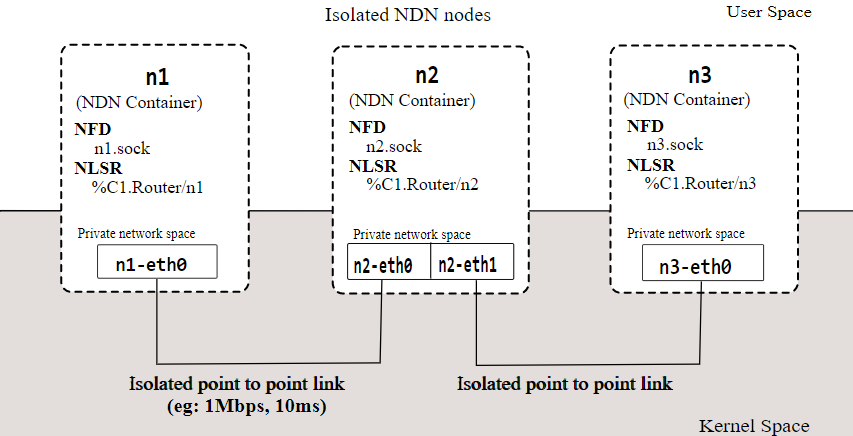
\includegraphics[width=6in]{minindn}
\caption{Basic MiniNDN architecture[memphis.edu]}
\end{figure}

\section{The Data Structure}
There are two data structures which were designed for the scope of this projects. These are the PibBlock and PibBlockchain. The PibBlockchain maintains a vector of hashed PibBlocks. It can return, at an index, a particular hashed block. It is maintained by the Public Information Base. 

The PibBlock class deals with the Certificates. It stores all information about a certificate as well as its version and the hash of the previous block.
\subsection{Public Information Base Block}
This is the basic building block of the PibBlockchain. It contains the current block's hash, certificate, version and timestamp as well as the previous block's hash. Mining the block is also done in the block class. The difficulty of the block mining is determined by the proof of work algorithm which takes in a a difficulty argument which determines how many zeroes need to be mined by the algorithm until a block is valid. For the purposes and scope of this project however, this algorithm wasn't fully implemented. 

The PibBlocks's constructor returns a pointer to a PibBlock's location in memory. For the initial Block, the PibBlock constructor takes no arguments and creates the genesis block which is based on a nonce cert. This is because we need to have an initial block with which we can hash the rest of the blocks. This bit of design wasn't particularly necessary as mentioned previously, the hashing algorithm wasn't implemented fully in the first place. 

Because the PibBlock class doesn't use smart pointers(more on this later), the class must have an explicitly defined destructor. In this destructor, all of the PibBlock's components are deleted. It is however important to note that the PibBlock's destructor doesn't correlate to the PibBlock's invalidator. Once created, a PibBlock cannot be destroyed or it will invalidate the whole Blockchain. Instead, there is an invalidator function, which simply sets the version of a PibBlock to 0 to imply that it has been invalidated. If the same certificate needs to be validated again, it must go through the whole proof of work process and be hashed to a new block with a version number 1.

Perhaps the most important design element of the PibBlock was the displaying of information. Early iterations would have each PibBlock copy a certificate onto a new certificate instance before adding the Block to the Blockchain. This proved disastrous as NFD does not allow certificates that haven't been signed by the KeyChain to exist, and if any are found the NDN network is shut down immediately.
\subsection{Public Information Base Blockchain}

Public Information Base(PIB) - This is the public key infrastructure hierarchy where identities are stored. Each identity in a network contains within it a default key and a default certificate. The counterpart private key information is stored in the Trusted Platform Module(TPM). We do not concern ourselves with the TPM as we only need the public keys to verify a node's signature. This is standard security procedure in any network. 

The PIB class in the NDN-CXX library is responsible for creating and publishing certificates. The design suggested by Dr. Weber was to create a wrapper so that any time a certificate is created, we could simply add it to the blockchain. Then the miner nodes could verify it and publish the given information. This however proved challenging in a number of ways. 

The first issue I encountered had to do with instancing. Because we needn't necessarily have only one instance of a PIB, we have to make sure that each PIB's certificates go in that specific PIB's Blockchain. This is precisely why Alexander Afanasyev has designed the PIB class in a way that one cannot instantiate a Trusted Platform Module(TPM) outside the PIB class i.e. the constructor for the PIB is the only place where the TPM is also constructed. This means that we cannot have a PIB be matched with a TPM that isn't its counter part. I aimed to achieve the same goal. I did this by looking outside of the PIB class. The PIB class is instantiated and governed by the KeyChain class. This in turn means that the KeyChain class instantiates both the PIB and the TPM. This is why I tried to make the constructor for the PibBlockchain data type to use as an argument the KeyChain's address meaning it would be instantiated in the KeyChain with code that looks something like "PibBlockchain certChain = new PibBlockchain(this);"

However, the PIB Blockchain was comprised of blocks or PibBlocks, which were a separate data structure which made use of the Certificates class in order to store certificates or indeed to be able to parse them at all in the first place. Because PibBlock inherited from Certificates, and PibBlockchain inherited from PibBlock and KeyChain inherited from both PibBlockchain and Certificates, there was suddenly a circular dependency which could not be broken without completely scrapping the PibBlockchain constructor design which takes a pointer to the KeyChain as an argument. 

\begin{figure}
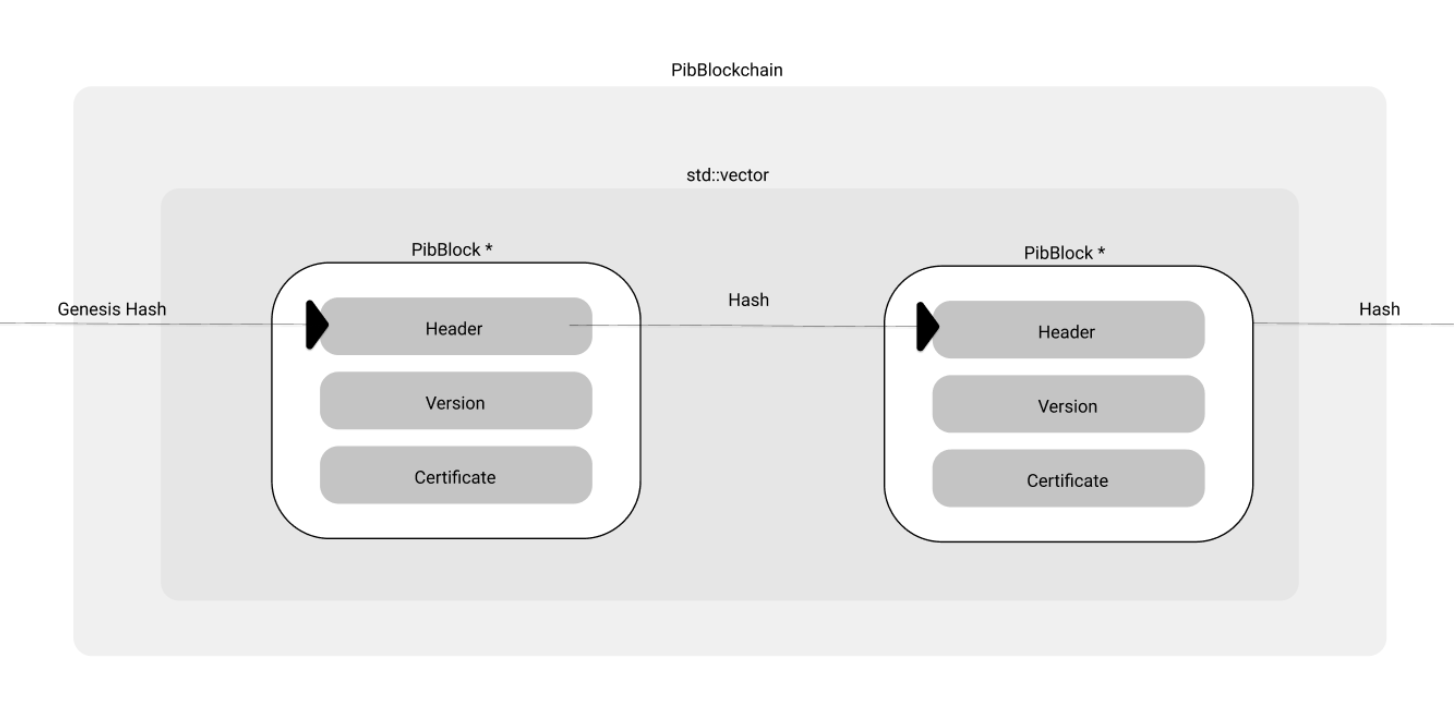
\includegraphics[width=6in]{pibblockchain.png}
\caption{This figure shows how PibBlockchain interacts with NDN and the std library}
\end{figure}

This is where Dr. Weber's original "wrapper" idea came to mind and to good use. Instead of having to worry about the KeyChain pointing to the correct PibBlockchain for each PIB, we could just instead make a mutable PibBlockchain in the PIB class which would work on the exact same principle as Alex Afanasyev's idea to instantiate the TPM in the PIB. We simply do the same thing with the PibBlockchain and instantiate it in the PIB. This way, we no longer have to worry having mismatched PIB and Blockchain. 

Blocks on the other hand weren't at all a concern when it came to creating instances of the Blockchain. The purpose of the PibBlock class is twofold: Firstly, to encapsulate all of the data from each Certificate and secondly, to do all of the "heavy lifting". What this means is that the PibBlock class is responsible for the hashing of each block. 

Of course this doesn't mean that there isn't a concern about which blocks go in which Blockchain. However, blocks are only created when Certificates are created. Certificates are created in the KeyChain.cpp. This means that each KeyChain has only one PibBlockchain to work with, because each KeyChain only instantiates one PIB. One PIB = One PibBlockchain. Therefore if we create PibBlocks in the KeyChain they will inherently be PibBlockchain specific and will be out of scope for any other KeyChains or PibBlockchains. This inherent property of C++ and indeed all object oriented programming made the challenge of making sure that each PibBlock is added to the correct Blockchain very simple.

"Within C++, there is a much smaller and clearer language struggling to get out" - Bjarne Soustroup[cit needed]
\\


Now that the allocation of PibBlocks to PibBlockchains was completed, and there were no longer any circular dependencies allowing for the code to be added to the security code hierarchy in NDN-CXX. \par 

Shortly after adding the code to the project, it became evident that the solution wouldn't work in its current form. That is because the NDN Team have developed a pretty robust automatic Certificate Authority. I found this out when I realized that my PibBlock data structure was parsing certificates being created, allocating new memory for them and then copying the certificate. The problem with this approach is that the copied certificates have not been authorised by the Certificate Authority. This is why when running the simulation, it would abruptly exit. 

So instead, the PibBlock class looks to the Certificate class for inspiration. The Certificate class overloads the << operator for certs by extracting all data from them and printing it in chunks. PibBlock takes the functions used to extract data from the certificates and implements them in order to store the Certificate data in strings. Once stored, nodes can still access the signatures for each certificate in string form and verify them.
\vfill
\begin{figure}[h]
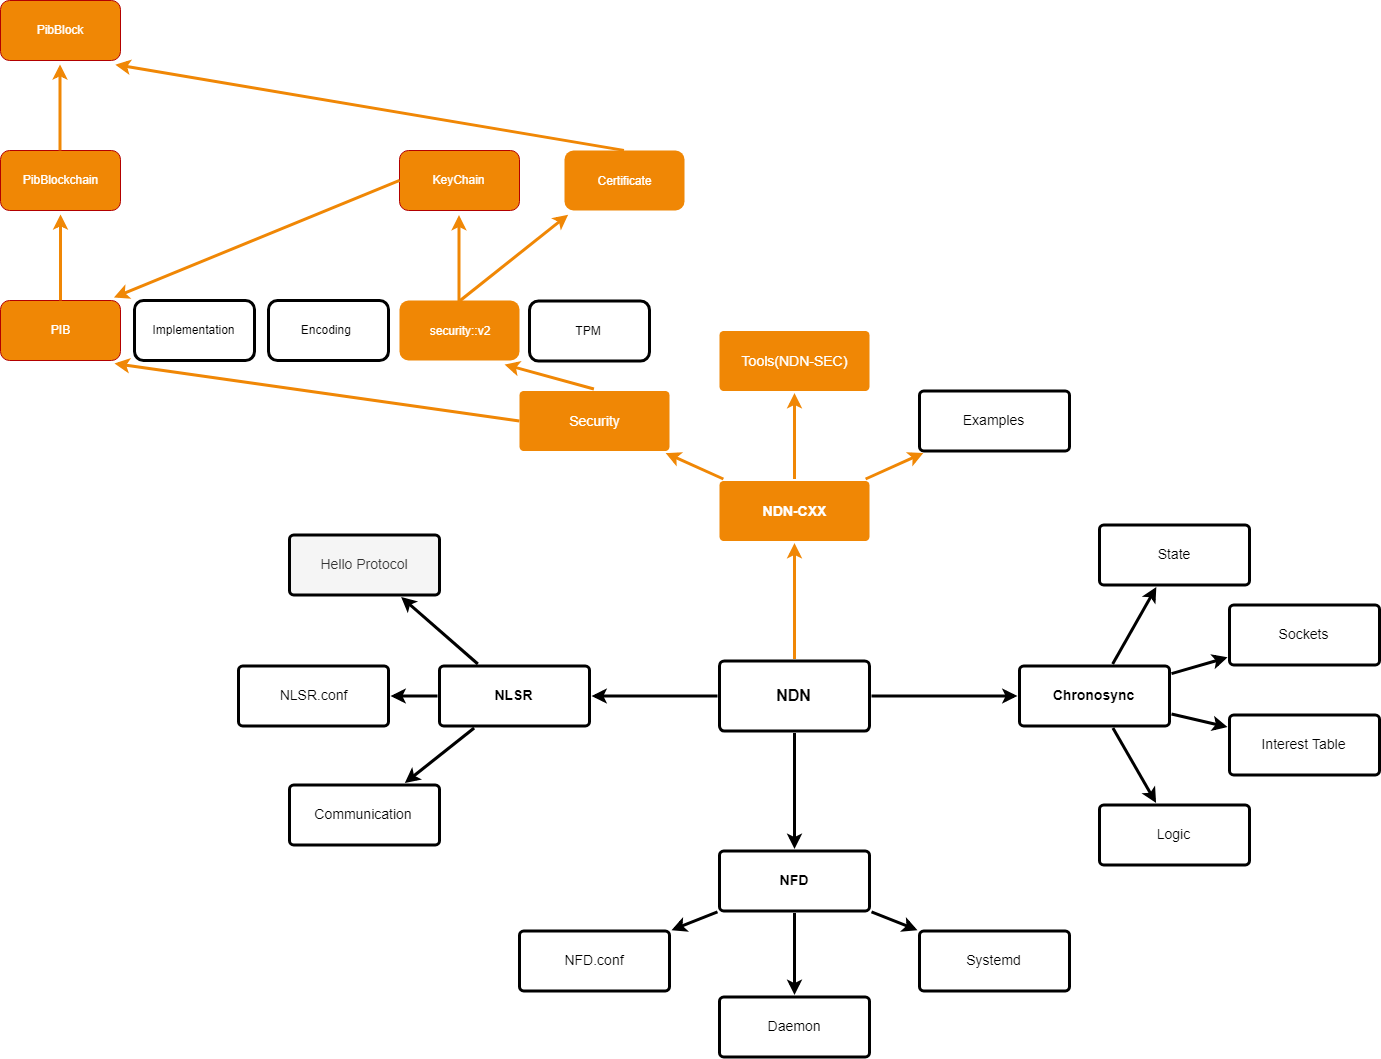
\includegraphics[width=6in]{NDN.png}
\caption{
NDN Components.Orange Rectangles - Intimate knowledge of modules' code required. Orange Rectangles w/ Red Frames - Modules where code was either altered or added for the scope of this project.}
\end{figure}
\section{Broadcasting}
Once the data is stored in the Blockchain, the next objective was to figure out a way to disseminate it across the network. This is the most important part of the project. The reason why the Blockchain is useful is so nodes can compare certificates against it. If they can't do that because they don't have that information, then the Blockchain is useless. The reason why the solution required was non-trivial was because of the communications design in NDN. In order for nodes to communicate, they must send out an Interest - which made the tasks more difficult than anticipated. \par 
\begin{figure}[h]
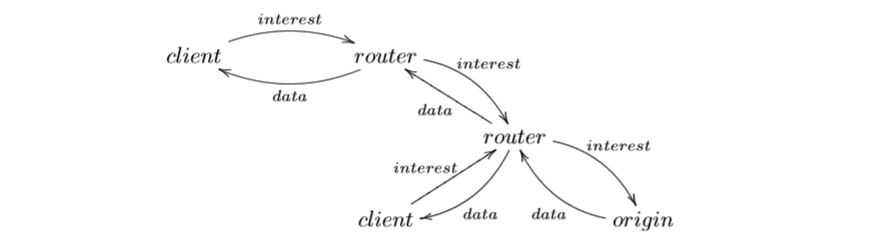
\includegraphics[width=6in]{comms.png}
\caption{Node Communication[A Survey of ICN - Dirk Kutscher]}
\end{figure}
\subsection{Naive Approach}
The proof of concept method of broadcasting the blockchain on port (ask Stefan for port no.) utilizes, in the case of MiniNDN, the file system. The Blockchain is broadcast to all nodes via the port and appears in the temp folder for all of the nodes. This is the naive approach and it is impractical because it just blasts data at the nodes and wouldn't work in a real environment.

\subsection{Reconfigure NFD approach}
The NFD is, as mentioned in the previous chapter, how Data and Interest packets get propagated in an NDN network. While investigating different options for broadcasting, I came across the configuration file for NFD which gives the user the option to redefine all nodes' caching policies. In it, there are a couple of listed policies. One only allows Data packets to be cached for which there are expressed Interests. The other allows Data to be cached regardless of whether there's been an Interest for it. \par
This project has explored one option for this approach. Because reconfiguring the NFD to make it so every node caches everything isn't feasible or wise, the option to create an altogether new policy was explored. However, there wasn't enough time to explore this option fully.
\subsection{Signed Interest approach}
This is the approach which was chosen for this project. Firstly, we must define a Signed Interest. This type of Interest is the second version of what was known as a "Control Interest". These specialized Interest packets were designed for Internet Of Things applications where nodes would have to communicate and sometimes control one another and the conventional Interest-Data packet communication didn't allow for this.\par

In a control system where a thermometer node has to tell a WiFi connected HVAC the temperature, so it can adjust accordingly, the conventional system leads to a paradox. This is because the thermometer node cannot simply send a Data packet to the HVAC, giving it the temperature, because this Data packet would be unsolicited. Also, it is not feasible to set up the HVAC to flood the network with temperature Interest packets at all times because this creates unnecessary strain on the network. It would be quite pointless to send out Interests(polling) at a random or set interval as well, as in most environments, temperature change doesn't happen at set intervals. This could make for an ineffective temperature control system if the temperature has changed from the desired temperature but the HVAC isn't due to poll the thermometer for a prolonged amount of time. \par 
Instead, the thermometer node sends a "Control Interest"(now deprecated and known instead as a Signed Interest) where it tells the HVAC to ask for the temperature reading.\par 
\begin{figure}
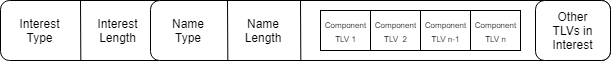
\includegraphics[width=6in]{signedinterest.png}
\caption{Signed Interest}
\end{figure}
We are met with a near identical situation. We have miners which need to broadcast a Blockchain to all nodes in a network. One approach could be to ensure that nodes request an updated Blockchain every time that they receive a Data packet. However, the delay from doing this would render the solution pointless and would provide little benefit in terms of a speed-up compared to the regular PIB look-up that nodes do(it would still improve on the single point of failure problem). So instead, when the miner verifies a new Certificate in the Blockchain, it sends out a Signed Interest to all nodes, to get them to request the information(Express an Interest) for the updated Blockchain. \par

The nodes in the network would have an InterestFilter which will verify that this Interest is indeed coming from an authenticated miner. Once the node receives the Signed Certificate, it will send an Interest packet to the miner to send out the updated Blockchain. This adds additional strain on the network, however, this is counterbalanced by the reduction in look-ups that nodes have to do in order to verify certificates.
  \chapter{Results}
\section{Ideal Evaluation}
\subsection{Overhead and Latency}
\section{Discussion}


  \chapter{Results}
This chapter presents the result of the Blockchain in NDN experiment. The outcome of this experiment is interesting because it presents a different approach to verifying certificates. This project recognizes that, despite the apparent benefits of not having to contact the Certificate Authority for verification, there is also added complexity to the NDN security protocol. The results from this experiment investigate the trade off in this scenario, in different topologies using MiniNDN. Because of the serious time constraint imposed by our different modules, this project instead presents an ideal evaluation for the experiment.
\section{Ideal Evaluation}
Because of time constraints, only very limited testing was done with this project. The ideal evaluation for the Blockchain however, would involve testing a number of different realistic topologies. Ideally, one would request a certificate from the NDN team for the ability to test on the official testbed. This would allow for realistic results which are desirable. There are a number of different topologies that must be tested including the `dumbbell' topology with two chokepoint routers. It is desirable to test different data sets, with different data sizes, and also different intervals of node communication. There must be a control experiment for each of the listed experiments. MiniNDN allows for huge amounts of configuration and customization for each node in a topology. A user can set different Hyperbolic Routing variables as well as delay and bandwidth between nodes and also links, allowing for extensive and robust network testing.
\begin{figure}[ht]
\centering
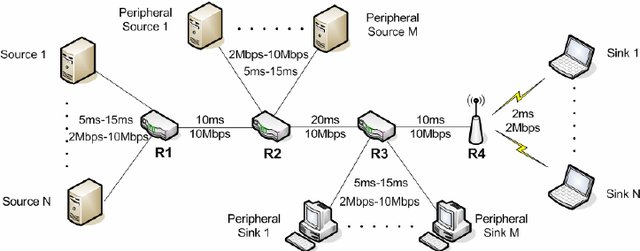
\includegraphics[scale=0.5]{topology.jpg}
\caption{Sample Topology \cite{057}}
\end{figure}

\begin{figure}
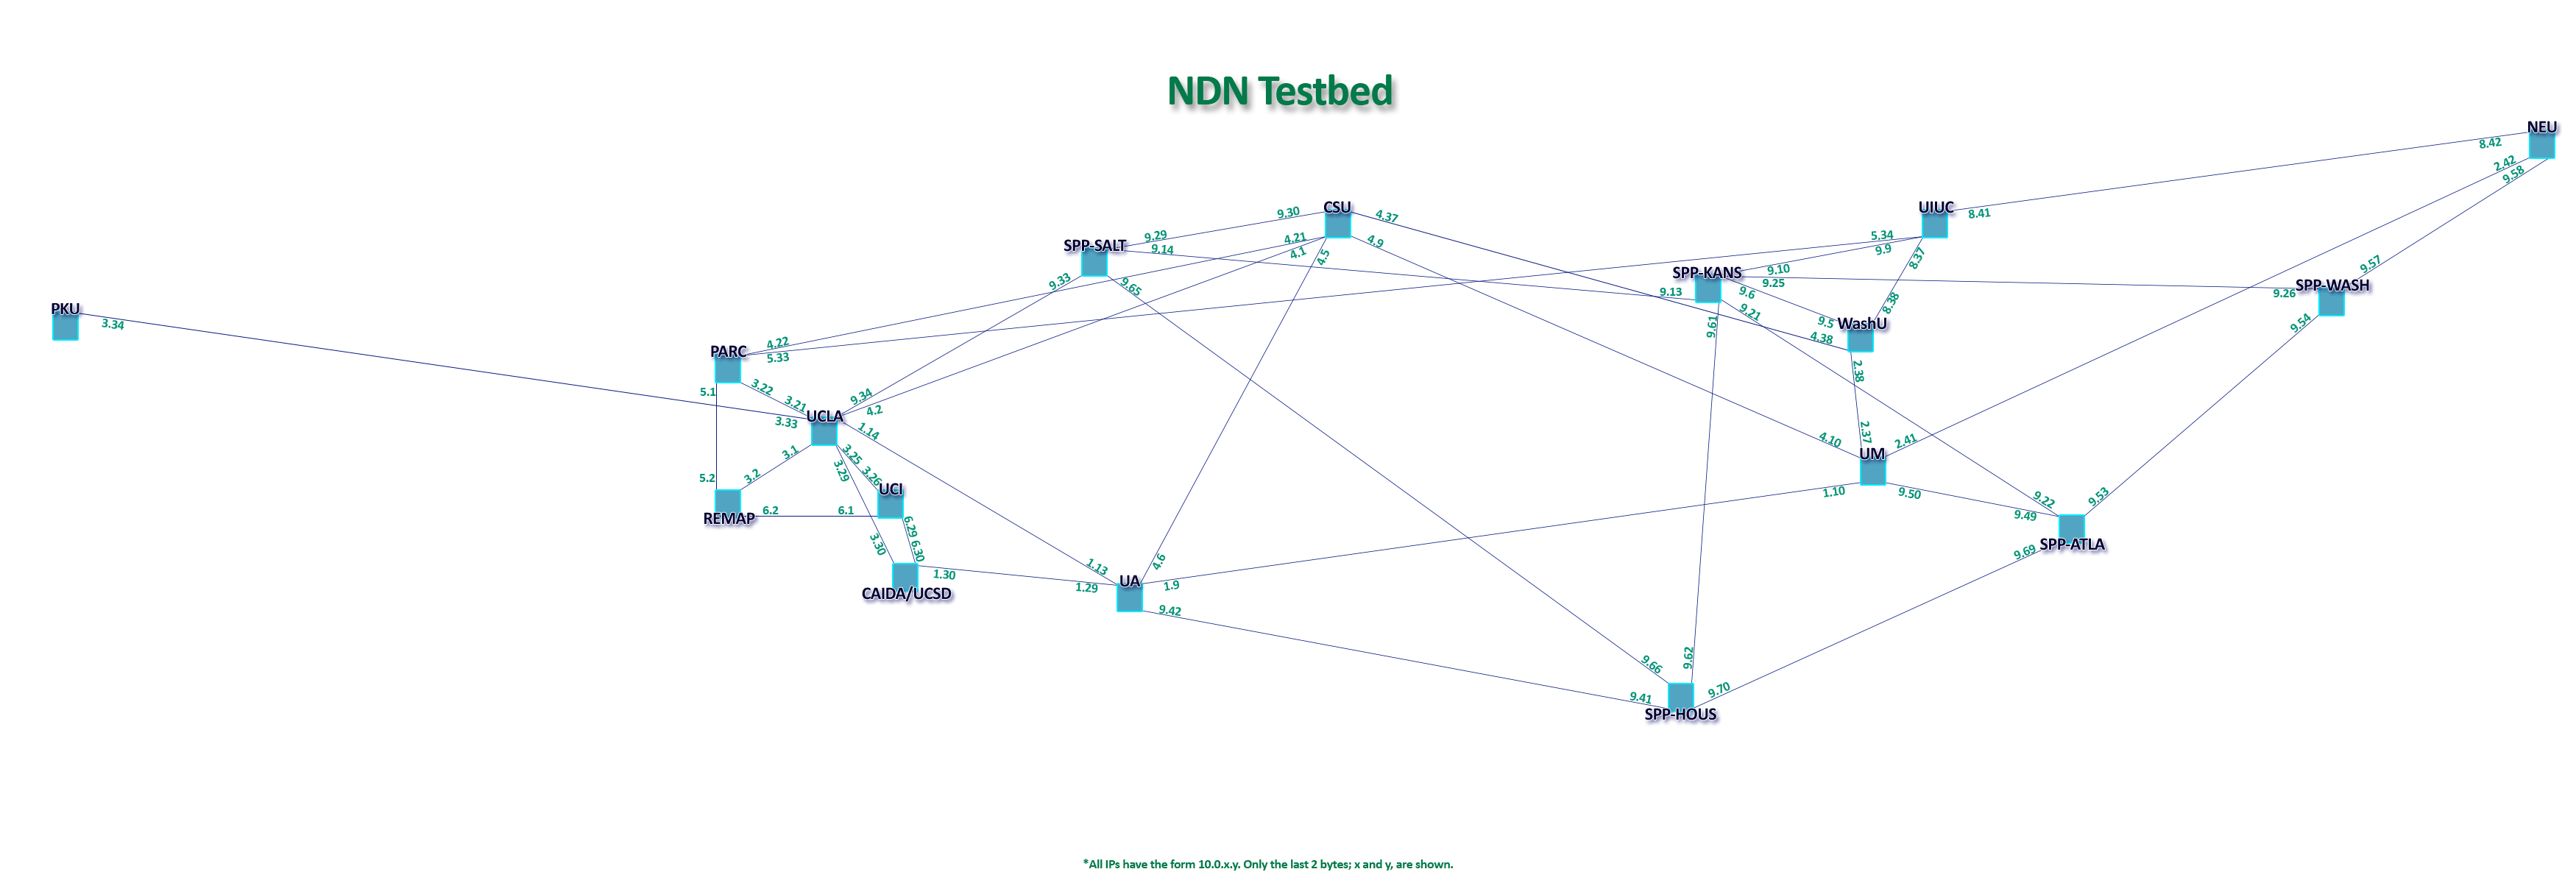
\includegraphics[width=6in]{topology.png}
\caption{The Current NDN Testbed Topology \cite{055}}
\end{figure}
\subsection{Overhead and Latency}
By increasing the complexity of NDN, one inadvertently adds overhead. The trade-off of that is the amount of time saved by nodes that don't have to communicate with the CA in order to verify Data. The concept itself works and isn't new. Browsers pre-install certificates to reduce look-up times. The idea here is to do the same by adding as little complexity as possible. And so, this project aims to achieve a golden ratio of complexity to efficiency. Adding the Blockchain data type to the NDN architecture adds bloat. If every node has that bit of overhead of having the Blockchain stored in its content store, it begs the question whether there's enough of a speed up from look-up reduction time to justify it. Especially seen as we are broadcasting the Blockchain, and some nodes might not be or want to be communicating at all. Yet, they are to request the Blockchain when the miners publish a Block.
\section{Discussion}
The evaluation of the success of this project greatly depends on whether one values a bigger Content Store or quicker communication between nodes. This is because every node would have to maintain the blocks in their cache. Blockchain in NDN greatly reduces communication with external Certificate Authorities. However, it can greatly add to the complexity of a network. Also, if it's a case of needing all nodes to have the Blockchain information simultaneously, then Chronosync is required, adding more complexity to the system. 

  \chapter{Results}
\section{Ideal Evaluation}
\subsection{Overhead and Latency}
\section{Discussion}


  \chapter{Conclusions}

And a fancy conclusion...



%\addcontentsline {toc}{chapter}{Appendices}       %% Force Appendices to appear in contents
\begin{appendix}
\chapter{Abbreviations}

\begin{longtable}{p{40mm}|p{100mm}}
	\textbf{Short Term}&\textbf{Expanded Term}\\
	\hline
	CA & Central Authority\\
	DNS & Domain Name System\\
	ACK & Packet Acknowledgement \\ 
	IoT & Internet of Things \\  
	URI & Universal Resource Indicator \\  
	ICN & Infomration Centric Networks\\ 
	NDN & Named Data Networking \\ 
	CCN & Content Centric Networking\\ 
	NDN-CXX & C++ Library with eXperimental eXtensions \\ 
	NFD & Named Data Forwarding Daemon \\ 
	NLSR & Named Data Link State Routing \\ 
	LSA & Link State Advertisement \\ 
	HR & Hyperbolic Routing \\  
	Face & Interface(Physical/Logical)\\ 
	FIB & Forward Interest Base \\ 
	CS & Content Store(Cache) \\ 
	PIT & Pending Interest Table \\ 
	PIB & Public Information Base \\ 
	RIB & Routing Information Base \\ 
	PKI & Public Key Infrastructure \\ 
	TPM & Trusted Platform Module \\ 
	TLV & Type Length Value Encoding \\ 
	TCP & Transmission Control Protocol \\ 
	IP & Internet Protocol  \\ 
	LNPM & Longest Name Prefix Matching \\
	DHCP & Dynamic Host Configuration Protocol \\ 
	ARP & Address Resolution Protocol \\ 
	DNS & Domain Name System \\ 
	MAC & Media Access Control \\ 
	RTT & Round Trip Time \\ 
\end{longtable}

%\chapter{Another appendix}

...

\end{appendix}


%\addcontentsline {toc}{chapter}{Bibliography}     %% Force Bibliography to appear in contents

\begin{thebibliography}{ieeetr}                   %% Start your bibliography here; you can
%\bibliography{refs}                               %% also use the \bibliography command



\bibitem{01}
[Zhang17a] ``An Overview of Named Data Networking by Lixia Zhang." Proceedings of
MILCOM 2017. Baltimore, MD, USA. Oct 2017.

\bibitem{02}
[Ioannou16] ``A Survey of Caching Policies and Forwarding Mechanisms in Information-Centric Networking" by Andrianna Ioannou \& Stefan Weber. IEEE Communications Surveys \& Tutorials. Volume:18, Issue:4, Q4 2016.

\bibitem{03}
[C.Index13] ``Cisco visual networking index: Forecast and methodology 2012-2017" by C. Index, White Paper. May 2013.


\bibitem{04}
[Kohnfelder78a] ``Towards a Practical Public-Key Cryptosystem" by Loren M. Kohnfelder. B.Sc. Dissertation. MIT, Boston, MA, USA, May 1978.

\bibitem{05}
[Kohnfelder78b] ``Towards a Practical Public-Key Cryptosystem" by Loren M. Kohnfelder. B.Sc. Dissertation. MIT, Boston, MA, USA, May 1978.

\bibitem{06}
[Weber19] ``Thesis first draft corrections" by Stefan Weber. TCD, Dublin, Apr 2019.

\bibitem{07}
[Nakamoto09a] ``Bitcoin: A Peer-to-Peer Electronic Cash System" by Satoshi Nakamoto, Oct 2008.  \texttt{\url{https://bitcoin.org/bitcoin.pdf}}

\bibitem{08}
[Nakamoto09b] ``Bitcoin: A Peer-to-Peer Electronic Cash System" by Satoshi Nakamoto, Oct 2008.  \texttt{\url{https://bitcoin.org/bitcoin.pdf}}


\bibitem{09}
[Nakamoto09c] ``Bitcoin: A Peer-to-Peer Electronic Cash System" by Satoshi Nakamoto, Oct 2008.  \texttt{url{https://bitcoin.org/bitcoin.pdf}}



\bibitem{010}
[Jacobson06a] ``A New Way to Look at Networking" by Van Jacobson. Google Tech Talks Archive, Aug 2006. \texttt{\url{https://youtu.be/oCZMoY3q2uM}}

\bibitem{011}
[Jacobson06b]  ``A New Way to Look at Networking" by Van Jacobson. Google Tech Talks Archive, Aug 2006. \texttt{\url{https://youtu.be/oCZMoY3q2uM}}


\bibitem{012}
[Medium] ``How The Byzantine General Sacked the Castle - A Look into Blockchain" by Debraj Ghosh. Medium.com, Apr 2016.


\bibitem{013}
[Shostack82] ``The Byzantine Generals Problem" by L. Lamport, R.Shostack \& M. Pease. ACM Transactions on Programming Languages and Systems, Vol. 4, No. 3. Jul 1982.


\bibitem{014}
[Nakamoto09d] ``Bitcoin: A Peer-to-Peer Electronic Cash System" by Satoshi Nakamoto, Oct 2008.  \texttt{\url{https://bitcoin.org/bitcoin.pdf}}


\bibitem{015}
[Nakamoto09e] ``Bitcoin: A Peer-to-Peer Electronic Cash System" by Satoshi Nakamoto, Oct 2008.  \texttt{\url{https://bitcoin.org/bitcoin.pdf}}


\bibitem{016}
[Zhang17b] ``An Overview of Named Data Networking by Lixia Zhang." Proceedings of
MILCOM 2017. Baltimore, MD, USA, Oct 2017. 

\bibitem{017}
[Zhang14] ``Named Data Networking" by Lixia Zhang, Van Jacobson \& Alexander Afanasyev. Proceedings of ACM SIGCOMM 2014. Chicago, IL, USA, Aug 2014.

\bibitem{018}
[Named-Data.net] ``Name Docs" by NDN Team. NDN Packet Format Specification. \texttt{\url{https://named-data.net/doc/NDN-packet-spec/current/name.html}}

\bibitem{019}
[Yuan15a] ``Reliably Scalable Name Prefix Lookup" by Haowei Yuan \& Patrick Crowley.Proceedings of ACM/IEEE Symposium on Architectures for Networking and Communication Systems(ANCS 2015). Oakland, CA, USA.	May 2015.

\bibitem{020}
[Wikipedia] ``Example for Longest Prefix Matching." \texttt{\url{https://en.wikipedia.org/wiki/Longest_prefix_match}}

\bibitem{021}
[Yuan15b] ``Reliably Scalable Name Prefix Lookup" by Haowei Yuan \& Patrick Crowley.Proceedings of ACM/IEEE Symposium on Architectures for Networking and Communication Systems(ANCS 2015). Oakland, CA, USA.	May 2015.

\bibitem{022}
[Yuan15c] ``Reliably Scalable Name Prefix Lookup" by Haowei Yuan \& Patrick Crowley.Proceedings of ACM/IEEE Symposium on Architectures for Networking and Communication Systems(ANCS 2015). Oakland, CA, USA.	May 2015.

\bibitem{023}
[Rainer18a] ``Challenges and Opportunities of Named Data Networking in Vehicle-To-Everything Communication: A Review" by Benjamin Rainer \& Stefan Petscharing. Center for Safety and Communications Technologies, Austrian Institute of Technology. Vienna, Austria. October 2018.


\bibitem{024}
[ndn-docs] ``Face Class" by NDN Team. NDN Common Client Libraries API 0.6.5. documentation. \texttt{\url{https://named-data.net/doc/ndn-ccl-api/face.html}}

\bibitem{025}
[V2E paperb] ``Challenges and Opportunities of Named Data Networking in Vehicle-To-Everything Communication: A Review" by Benjamin Rainer \& Stefan Petscharing. Center for Safety and Communications Technologies, Austrian Institute of Technology. Vienna, Austria. October 2018.



\bibitem{026}
[V2E paperc] ``Challenges and Opportunities of Named Data Networking in Vehicle-To-Everything Communication: A Review" by Benjamin Rainer \& Stefan Petscharing. Center for Safety and Communications Technologies, Austrian Institute of Technology. Vienna, Austria. October 2018.


\bibitem{027}
[Jacobson09a] ``Networking Named Content" by Van Jacobson, Diana Smetters, James Thornton, Michael Plass, Nicholas Briggs \& Rebecca Braynard. Proceedings of the \nth{5} International Conference on Emerging Networking Experiments and Technologies. Rome, Italy. December 2009.

\bibitem{028}
[Jacobson09b] ``Networking Named Content" by Van Jacobson, Diana Smetters, James Thornton, Michael Plass, Nicholas Briggs \& Rebecca Braynard. Proceedings of the \nth{5} International Conference on Emerging Networking Experiments and Technologies. Rome, Italy. December 2009.

\bibitem{029}
[NFDTeam16] ``NFD Developer's Guide" by the NFD Team. NDN Technical Report, NDN-0021. Oct 2016.

\bibitem{030}
[Wang18a] ``A Secure Link State Routing Protocol for NDN" by Lan Wang, Vince Lehman, A.K.M. Mahmudul Hoque, Beichuan Zhang, Yingdi Yu \& Lixia Zhang. In IEEE Access, Vol. 6. Jan 2018.

\bibitem{031}
[Wang18b] ``A Secure Link State Routing Protocol for NDN" by Lan Wang, Vince Lehman, A.K.M. Mahmudul Hoque, Beichuan Zhang, Yingdi Yu \& Lixia Zhang. In IEEE Access, Vol. 6. Jan 2018.


\bibitem{032}
[Wang18c] ``A Secure Link State Routing Protocol for NDN" by Lan Wang, Vince Lehman, A.K.M. Mahmudul Hoque, Beichuan Zhang, Yingdi Yu \& Lixia Zhang. In IEEE Access, Vol. 6. Jan 2018.
 


\bibitem{033}
[Wang18d] ``A Secure Link State Routing Protocol for NDN" by Lan Wang, Vince Lehman, A.K.M. Mahmudul Hoque, Beichuan Zhang, Yingdi Yu \& Lixia Zhang. In IEEE Access, Vol. 6. Jan 2018.
 


\bibitem{034}
[Wang18e] ``A Secure Link State Routing Protocol for NDN" by Lan Wang, Vince Lehman, A.K.M. Mahmudul Hoque, Beichuan Zhang, Yingdi Yu \& Lixia Zhang. In IEEE Access, Vol. 6. Jan 2018.
 

\bibitem{035}
[Wang18f] ``A Secure Link State Routing Protocol for NDN" by Lan Wang, Vince Lehman, A.K.M. Mahmudul Hoque, Beichuan Zhang, Yingdi Yu \& Lixia Zhang. In IEEE Access, Vol. 6. Jan 2018.
 

\bibitem{036}
[Afanasyev13a] ``Let's ChronoSync: Decentralized Dataset State
Synchronization in Named Data Networking" by Alexander Afanasyev \& Zhenkai Zhu.Proceedings of \nth{21} IEEE International Conference on Network Protocols(ICNP 2013).Göttingen, Germany. Oct 2013.


\bibitem{037}
[Afanasyev13b] ``Let's ChronoSync: Decentralized Dataset State
Synchronization in Named Data Networking" by Alexander Afanasyev \& Zhenkai Zhu.Proceedings of \nth{21} IEEE International Conference on Network Protocols(ICNP 2013).Göttingen, Germany. Oct 2013.


\bibitem{038}
[Ioannou14a] ``Towards On-Path Caching Alternatives in Information-Centric Networks" by Andrianna Ioannou \& Stefan Weber. Proceedings of 39th Annual IEEE Conference on Local Computer Networks. Edmonton, AB, Canada. Sept 2014.


\bibitem{039}
[Weber15] ``Towards On-Path Caching Alternatives in Information-Centric Networks" by Andrianna Ioannou \& Stefan Weber. Proceedings of 39th Annual IEEE Conference on Local Computer Networks. Edmonton, AB, Canada. Sept 2014.


\bibitem{040}
[Merkle79a] ``Protocols for Public-Key Cryptosystems" by Ralph Merkle. In 1980 IEEE Symposium on Security and Privacy. Oakland, CA, USA. Apr 1980.

\bibitem{041}
[Spyridon18a] ``An Overview of Security Support in Named Data Networking" by Spyridon Mastorakis, Zhiyi Zhang, Yingdi Yu, Haitao Zhang, Eric Newberry, Yanbiao Li, Alexander Afanasyev \& Lixia Zhang. NDN Technical Report, NDN-0057, Rev. 2. Apr. 2018.
\bibitem{042}
[Spyridon18b] ``An Overview of Security Support in Named Data Networking" by Spyridon Mastorakis, Zhiyi Zhang, Yingdi Yu, Haitao Zhang, Eric Newberry, Yanbiao Li, Alexander Afanasyev \& Lixia Zhang. NDN Technical Report, NDN-0057, Rev. 2. Apr. 2018.

\bibitem{043}
[Spyridon18c] ``An Overview of Security Support in Named Data Networking" by Spyridon Mastorakis, Zhiyi Zhang, Yingdi Yu, Haitao Zhang, Eric Newberry, Yanbiao Li, Alexander Afanasyev \& Lixia Zhang. NDN Technical Report, NDN-0057, Rev. 2. Apr. 2018.

\bibitem{044}
[Spyridon18d] ``An Overview of Security Support in Named Data Networking" by Spyridon Mastorakis, Zhiyi Zhang, Yingdi Yu, Haitao Zhang, Eric Newberry, Yanbiao Li, Alexander Afanasyev \& Lixia Zhang. NDN Technical Report, NDN-0057, Rev. 2. Apr. 2018.

\bibitem{045}
[Spyridon18e] ``An Overview of Security Support in Named Data Networking" by Spyridon Mastorakis, Zhiyi Zhang, Yingdi Yu, Haitao Zhang, Eric Newberry, Yanbiao Li, Alexander Afanasyev \& Lixia Zhang. NDN Technical Report, NDN-0057, Rev. 2. Apr. 2018.


\bibitem{046}
[Spyridon18f] ``An Overview of Security Support in Named Data Networking" by Spyridon Mastorakis, Zhiyi Zhang, Yingdi Yu, Haitao Zhang, Eric Newberry, Yanbiao Li, Alexander Afanasyev \& Lixia Zhang. NDN Technical Report, NDN-0057, Rev. 2. Apr. 2018.


\bibitem{047}
[Spyridon18g] ``An Overview of Security Support in Named Data Networking" by Spyridon Mastorakis, Zhiyi Zhang, Yingdi Yu, Haitao Zhang, Eric Newberry, Yanbiao Li, Alexander Afanasyev \& Lixia Zhang. NDN Technical Report, NDN-0057, Rev. 2. Apr. 2018.


\bibitem{048}
[Merkle79b]  ``Protocols for Public-Key Cryptosystems" by Ralph Merkle. In 1980 IEEE Symposium on Security and Privacy. Oakland, CA, USA. Apr 1980.


\bibitem{049}
[memphis.edu] ``What is MiniNDN?" by University of Memphis. \texttt{\url{http://minindn.memphis.edu/}}

\bibitem{050}
[Soustroup] ``The Design and Evolution of C++". pp. 207.

\bibitem{051}
[Kutscher15] ``A Survey of Information-Centric Networking" by Dirk Kutscher,  Börje Ohlman, Claudio Imbrenda, Christian Dannewitz \& Bengt Ahlgren. In IEEE Communications Magazine Vol. 50, No. 7. July 2012.

\bibitem{052}
[Afanasyev13c]``Let's ChronoSync: Decentralized Dataset State
Synchronization in Named Data Networking" by Alexander Afanasyev \& Zhenkai Zhu.Proceedings of \nth{21} IEEE International Conference on Network Protocols(ICNP 2013).Göttingen, Germany. Oct 2013.

\bibitem{053}
[Wang18g] ``A Secure Link State Routing Protocol for NDN" by Lan Wang, Vince Lehman, A.K.M. Mahmudul Hoque, Beichuan Zhang, Yingdi Yu \& Lixia Zhang. In IEEE Access, Vol. 6. Jan 2018.


\bibitem{054}
[Wang18h] ``A Secure Link State Routing Protocol for NDN" by Lan Wang, Vince Lehman, A.K.M. Mahmudul Hoque, Beichuan Zhang, Yingdi Yu \& Lixia Zhang. In IEEE Access, Vol. 6. Jan 2018.
 

\bibitem{055}
[Wang18i] ``A Secure Link State Routing Protocol for NDN" by Lan Wang, Vince Lehman, A.K.M. Mahmudul Hoque, Beichuan Zhang, Yingdi Yu \& Lixia Zhang. In IEEE Access, Vol. 6. Jan 2018.
 

\bibitem{056}
[Wang18j] ``A Secure Link State Routing Protocol for NDN" by Lan Wang, Vince Lehman, A.K.M. Mahmudul Hoque, Beichuan Zhang, Yingdi Yu \& Lixia Zhang. In IEEE Access, Vol. 6. Jan 2018.

\bibitem{057}
[Papadimitriou09] ``Real Time Video Streaming over Heterogeneous Networks" by Panagiotis Papadimitriou \& Vassilis Tsaussidis. Proceedings of \nth{11} International Conference On Advanced Communication Technology, 2009(ICACT 2009).Gangwon-Do, South Korea. Feb 2009.


\end{thebibliography}                             %% to generate your bibliography.


\end{document}                                    %% END THE DOCUMENT
